\documentclass[twoside]{book}

% Packages required by doxygen
\usepackage{fixltx2e}
\usepackage{calc}
\usepackage{doxygen}
\usepackage{graphicx}
\usepackage[utf8]{inputenc}
\usepackage{makeidx}
\usepackage{multicol}
\usepackage{multirow}
\PassOptionsToPackage{warn}{textcomp}
\usepackage{textcomp}
\usepackage[nointegrals]{wasysym}
\usepackage[table]{xcolor}

% Font selection
\usepackage[T1]{fontenc}
\usepackage{mathptmx}
\usepackage[scaled=.90]{helvet}
\usepackage{courier}
\usepackage{amssymb}
\usepackage{sectsty}
\renewcommand{\familydefault}{\sfdefault}
\allsectionsfont{%
  \fontseries{bc}\selectfont%
  \color{darkgray}%
}
\renewcommand{\DoxyLabelFont}{%
  \fontseries{bc}\selectfont%
  \color{darkgray}%
}
\newcommand{\+}{\discretionary{\mbox{\scriptsize$\hookleftarrow$}}{}{}}

% Page & text layout
\usepackage{geometry}
\geometry{%
  a4paper,%
  top=2.5cm,%
  bottom=2.5cm,%
  left=2.5cm,%
  right=2.5cm%
}
\tolerance=750
\hfuzz=15pt
\hbadness=750
\setlength{\emergencystretch}{15pt}
\setlength{\parindent}{0cm}
\setlength{\parskip}{0.2cm}
\makeatletter
\renewcommand{\paragraph}{%
  \@startsection{paragraph}{4}{0ex}{-1.0ex}{1.0ex}{%
    \normalfont\normalsize\bfseries\SS@parafont%
  }%
}
\renewcommand{\subparagraph}{%
  \@startsection{subparagraph}{5}{0ex}{-1.0ex}{1.0ex}{%
    \normalfont\normalsize\bfseries\SS@subparafont%
  }%
}
\makeatother

% Headers & footers
\usepackage{fancyhdr}
\pagestyle{fancyplain}
\fancyhead[LE]{\fancyplain{}{\bfseries\thepage}}
\fancyhead[CE]{\fancyplain{}{}}
\fancyhead[RE]{\fancyplain{}{\bfseries\leftmark}}
\fancyhead[LO]{\fancyplain{}{\bfseries\rightmark}}
\fancyhead[CO]{\fancyplain{}{}}
\fancyhead[RO]{\fancyplain{}{\bfseries\thepage}}
\fancyfoot[LE]{\fancyplain{}{}}
\fancyfoot[CE]{\fancyplain{}{}}
\fancyfoot[RE]{\fancyplain{}{\bfseries\scriptsize Generated on Mon Dec 8 2014 00\+:16\+:49 for Project 2 by Doxygen }}
\fancyfoot[LO]{\fancyplain{}{\bfseries\scriptsize Generated on Mon Dec 8 2014 00\+:16\+:49 for Project 2 by Doxygen }}
\fancyfoot[CO]{\fancyplain{}{}}
\fancyfoot[RO]{\fancyplain{}{}}
\renewcommand{\footrulewidth}{0.4pt}
\renewcommand{\chaptermark}[1]{%
  \markboth{#1}{}%
}
\renewcommand{\sectionmark}[1]{%
  \markright{\thesection\ #1}%
}

% Indices & bibliography
\usepackage{natbib}
\usepackage[titles]{tocloft}
\setcounter{tocdepth}{3}
\setcounter{secnumdepth}{5}
\makeindex

% Hyperlinks (required, but should be loaded last)
\usepackage{ifpdf}
\ifpdf
  \usepackage[pdftex,pagebackref=true]{hyperref}
\else
  \usepackage[ps2pdf,pagebackref=true]{hyperref}
\fi
\hypersetup{%
  colorlinks=true,%
  linkcolor=blue,%
  citecolor=blue,%
  unicode%
}

% Custom commands
\newcommand{\clearemptydoublepage}{%
  \newpage{\pagestyle{empty}\cleardoublepage}%
}


%===== C O N T E N T S =====

\begin{document}

% Titlepage & ToC
\hypersetup{pageanchor=false,
             bookmarks=true,
             bookmarksnumbered=true,
             pdfencoding=unicode
            }
\pagenumbering{roman}
\begin{titlepage}
\vspace*{7cm}
\begin{center}%
{\Large Project 2 }\\
\vspace*{1cm}
{\large Generated by Doxygen 1.8.8}\\
\vspace*{0.5cm}
{\small Mon Dec 8 2014 00:16:49}\\
\end{center}
\end{titlepage}
\clearemptydoublepage
\tableofcontents
\clearemptydoublepage
\pagenumbering{arabic}
\hypersetup{pageanchor=true}

%--- Begin generated contents ---
\chapter{Hierarchical Index}
\section{Class Hierarchy}
This inheritance list is sorted roughly, but not completely, alphabetically\+:\begin{DoxyCompactList}
\item \contentsline{section}{Board}{\pageref{class_board}}{}
\begin{DoxyCompactList}
\item \contentsline{section}{Players}{\pageref{class_players}}{}
\end{DoxyCompactList}
\item \contentsline{section}{Check\+Winner}{\pageref{class_check_winner}}{}
\item \contentsline{section}{Board\+:\+:Invalid\+Input}{\pageref{class_board_1_1_invalid_input}}{}
\end{DoxyCompactList}

\chapter{Class Index}
\section{Class List}
Here are the classes, structs, unions and interfaces with brief descriptions\+:\begin{DoxyCompactList}
\item\contentsline{section}{\hyperlink{struct_board}{Board} }{\pageref{struct_board}}{}
\item\contentsline{section}{\hyperlink{struct_players}{Players} }{\pageref{struct_players}}{}
\end{DoxyCompactList}

\chapter{File Index}
\section{File List}
Here is a list of all files with brief descriptions\+:\begin{DoxyCompactList}
\item\contentsline{section}{\hyperlink{_8dep_8inc}{.\+dep.\+inc} }{\pageref{_8dep_8inc}}{}
\item\contentsline{section}{\hyperlink{main_8cpp}{main.\+cpp} }{\pageref{main_8cpp}}{}
\item\contentsline{section}{build/\+Debug/\+Cygwin\+\_\+4.\+x-\/\+Windows/\hyperlink{main_8o_8d}{main.\+o.\+d} }{\pageref{main_8o_8d}}{}
\end{DoxyCompactList}

\chapter{Class Documentation}
\hypertarget{class_board}{\section{Board Class Reference}
\label{class_board}\index{Board@{Board}}
}


{\ttfamily \#include $<$Board.\+h$>$}

Inheritance diagram for Board\+:\begin{figure}[H]
\begin{center}
\leavevmode
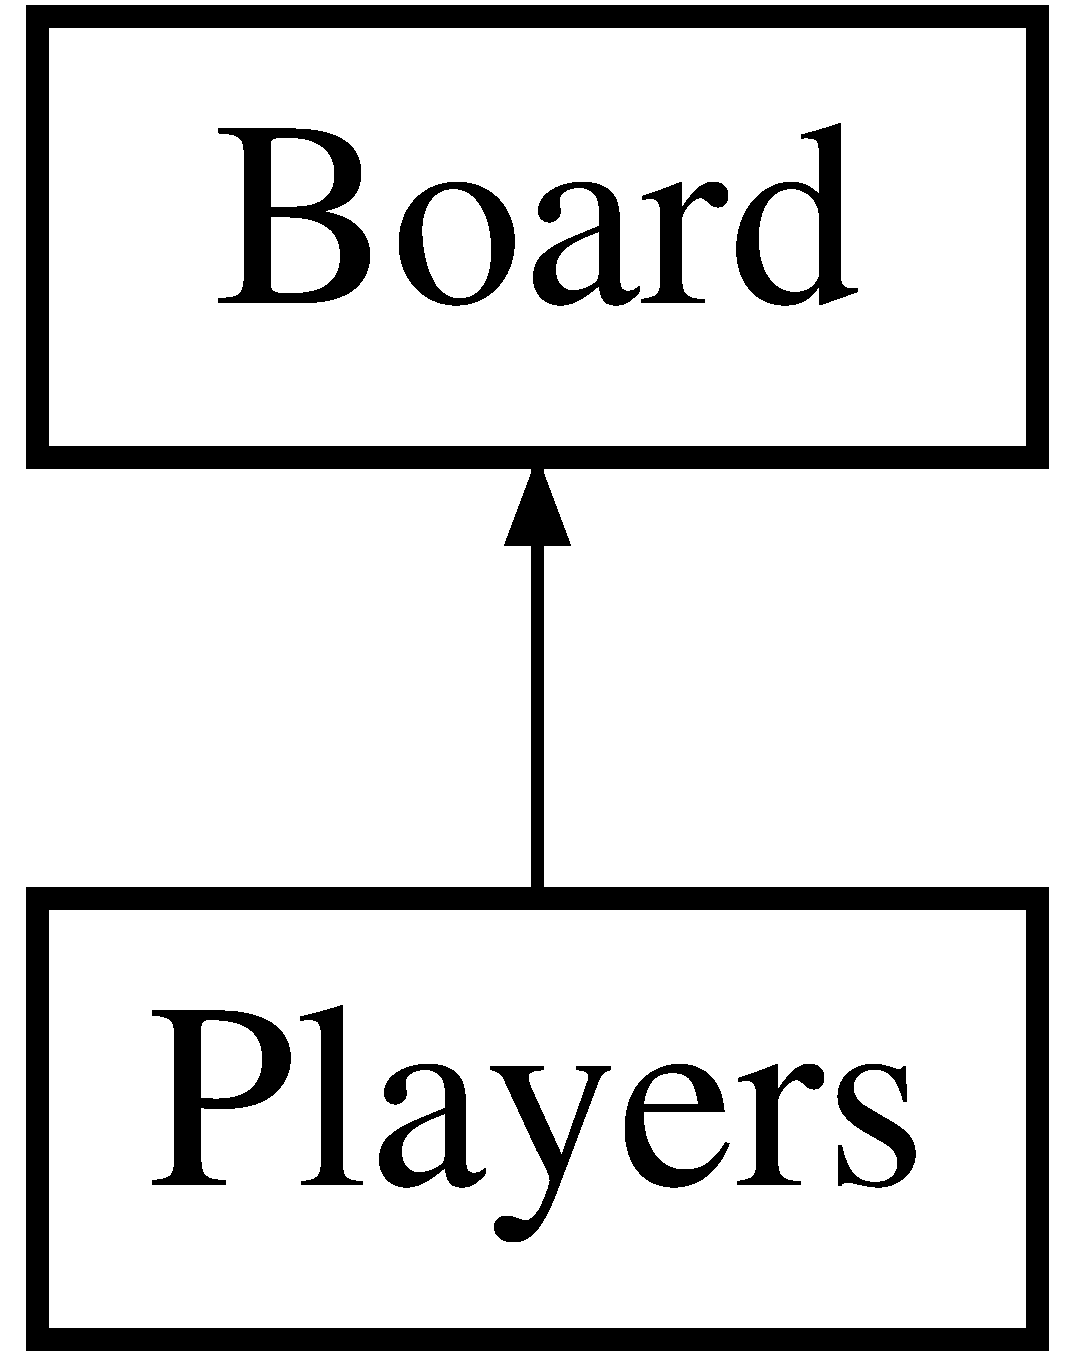
\includegraphics[height=2.000000cm]{class_board}
\end{center}
\end{figure}
\subsection*{Classes}
\begin{DoxyCompactItemize}
\item 
class \hyperlink{class_board_1_1_invalid_input}{Invalid\+Input}
\end{DoxyCompactItemize}
\subsection*{Public Member Functions}
\begin{DoxyCompactItemize}
\item 
\hyperlink{class_board_a9ee491d4fea680cf69b033374a9fdfcb}{Board} ()
\item 
\hyperlink{class_board_a299f62d90ba5fbdc8440bfe308b8a8aa}{Board} (int, int, int)
\item 
void \hyperlink{class_board_a6ad160481be18744397f962ee8e4d814}{set\+Rows} (int)
\item 
void \hyperlink{class_board_adccbab14197ba03304e799fe840e4992}{set\+Columns} (int)
\item 
void \hyperlink{class_board_aff7bda31a5f7cc05889b5ac1b81b2b7e}{set\+Ships} (int)
\item 
int \hyperlink{class_board_a80079a2b2bdec57b229bf110ce79c5ef}{get\+Rows} () const 
\item 
int \hyperlink{class_board_a2fafe4b1b84a90291594db2bef616619}{get\+Columns} () const 
\item 
int \hyperlink{class_board_a0a3f08f39f671639eacf531225b99eba}{get\+Ships} () const 
\end{DoxyCompactItemize}


\subsection{Detailed Description}


Definition at line 11 of file Board.\+h.



\subsection{Constructor \& Destructor Documentation}
\hypertarget{class_board_a9ee491d4fea680cf69b033374a9fdfcb}{\index{Board@{Board}!Board@{Board}}
\index{Board@{Board}!Board@{Board}}
\subsubsection[{Board}]{\setlength{\rightskip}{0pt plus 5cm}Board\+::\+Board (
\begin{DoxyParamCaption}
{}
\end{DoxyParamCaption}
)}}\label{class_board_a9ee491d4fea680cf69b033374a9fdfcb}


Definition at line 10 of file Board.\+cpp.

\hypertarget{class_board_a299f62d90ba5fbdc8440bfe308b8a8aa}{\index{Board@{Board}!Board@{Board}}
\index{Board@{Board}!Board@{Board}}
\subsubsection[{Board}]{\setlength{\rightskip}{0pt plus 5cm}Board\+::\+Board (
\begin{DoxyParamCaption}
\item[{int}]{r, }
\item[{int}]{c, }
\item[{int}]{s}
\end{DoxyParamCaption}
)}}\label{class_board_a299f62d90ba5fbdc8440bfe308b8a8aa}


Definition at line 16 of file Board.\+cpp.



\subsection{Member Function Documentation}
\hypertarget{class_board_a2fafe4b1b84a90291594db2bef616619}{\index{Board@{Board}!get\+Columns@{get\+Columns}}
\index{get\+Columns@{get\+Columns}!Board@{Board}}
\subsubsection[{get\+Columns}]{\setlength{\rightskip}{0pt plus 5cm}int Board\+::get\+Columns (
\begin{DoxyParamCaption}
{}
\end{DoxyParamCaption}
) const}}\label{class_board_a2fafe4b1b84a90291594db2bef616619}


Definition at line 52 of file Board.\+cpp.

\hypertarget{class_board_a80079a2b2bdec57b229bf110ce79c5ef}{\index{Board@{Board}!get\+Rows@{get\+Rows}}
\index{get\+Rows@{get\+Rows}!Board@{Board}}
\subsubsection[{get\+Rows}]{\setlength{\rightskip}{0pt plus 5cm}int Board\+::get\+Rows (
\begin{DoxyParamCaption}
{}
\end{DoxyParamCaption}
) const}}\label{class_board_a80079a2b2bdec57b229bf110ce79c5ef}


Definition at line 51 of file Board.\+cpp.

\hypertarget{class_board_a0a3f08f39f671639eacf531225b99eba}{\index{Board@{Board}!get\+Ships@{get\+Ships}}
\index{get\+Ships@{get\+Ships}!Board@{Board}}
\subsubsection[{get\+Ships}]{\setlength{\rightskip}{0pt plus 5cm}int Board\+::get\+Ships (
\begin{DoxyParamCaption}
{}
\end{DoxyParamCaption}
) const}}\label{class_board_a0a3f08f39f671639eacf531225b99eba}


Definition at line 53 of file Board.\+cpp.

\hypertarget{class_board_adccbab14197ba03304e799fe840e4992}{\index{Board@{Board}!set\+Columns@{set\+Columns}}
\index{set\+Columns@{set\+Columns}!Board@{Board}}
\subsubsection[{set\+Columns}]{\setlength{\rightskip}{0pt plus 5cm}void Board\+::set\+Columns (
\begin{DoxyParamCaption}
\item[{int}]{c}
\end{DoxyParamCaption}
)}}\label{class_board_adccbab14197ba03304e799fe840e4992}


Definition at line 35 of file Board.\+cpp.

\hypertarget{class_board_a6ad160481be18744397f962ee8e4d814}{\index{Board@{Board}!set\+Rows@{set\+Rows}}
\index{set\+Rows@{set\+Rows}!Board@{Board}}
\subsubsection[{set\+Rows}]{\setlength{\rightskip}{0pt plus 5cm}void Board\+::set\+Rows (
\begin{DoxyParamCaption}
\item[{int}]{r}
\end{DoxyParamCaption}
)}}\label{class_board_a6ad160481be18744397f962ee8e4d814}


Definition at line 31 of file Board.\+cpp.

\hypertarget{class_board_aff7bda31a5f7cc05889b5ac1b81b2b7e}{\index{Board@{Board}!set\+Ships@{set\+Ships}}
\index{set\+Ships@{set\+Ships}!Board@{Board}}
\subsubsection[{set\+Ships}]{\setlength{\rightskip}{0pt plus 5cm}void Board\+::set\+Ships (
\begin{DoxyParamCaption}
\item[{int}]{s}
\end{DoxyParamCaption}
)}}\label{class_board_aff7bda31a5f7cc05889b5ac1b81b2b7e}


Definition at line 39 of file Board.\+cpp.



The documentation for this class was generated from the following files\+:\begin{DoxyCompactItemize}
\item 
\hyperlink{_board_8h}{Board.\+h}\item 
\hyperlink{_board_8cpp}{Board.\+cpp}\end{DoxyCompactItemize}

\hypertarget{class_check_winner}{\section{Check\+Winner Class Reference}
\label{class_check_winner}\index{Check\+Winner@{Check\+Winner}}
}


{\ttfamily \#include $<$Check\+Winner.\+h$>$}

\subsection*{Public Member Functions}
\begin{DoxyCompactItemize}
\item 
\hyperlink{class_check_winner_a3fd98734824ee2f199ddbd82e09868c7}{Check\+Winner} ()
\item 
\hyperlink{class_check_winner_a85c10b3fb71bda10bffce29a1c9f67b2}{Check\+Winner} (int pl, int en)
\item 
void \hyperlink{class_check_winner_afd7b2c0a6c3f24d4edde68b08b34d294}{set\+Pl\+Points} (int pl)
\item 
void \hyperlink{class_check_winner_ad8aa4e5aea60c43e8fcf393da98e801a}{set\+En\+Points} (int en)
\item 
void \hyperlink{class_check_winner_a8e6c548984d215ed2af031255423161e}{get\+Result} ()
\end{DoxyCompactItemize}


\subsection{Detailed Description}


Definition at line 12 of file Check\+Winner.\+h.



\subsection{Constructor \& Destructor Documentation}
\hypertarget{class_check_winner_a3fd98734824ee2f199ddbd82e09868c7}{\index{Check\+Winner@{Check\+Winner}!Check\+Winner@{Check\+Winner}}
\index{Check\+Winner@{Check\+Winner}!Check\+Winner@{Check\+Winner}}
\subsubsection[{Check\+Winner}]{\setlength{\rightskip}{0pt plus 5cm}Check\+Winner\+::\+Check\+Winner (
\begin{DoxyParamCaption}
{}
\end{DoxyParamCaption}
)\hspace{0.3cm}{\ttfamily [inline]}}}\label{class_check_winner_a3fd98734824ee2f199ddbd82e09868c7}


Definition at line 18 of file Check\+Winner.\+h.

\hypertarget{class_check_winner_a85c10b3fb71bda10bffce29a1c9f67b2}{\index{Check\+Winner@{Check\+Winner}!Check\+Winner@{Check\+Winner}}
\index{Check\+Winner@{Check\+Winner}!Check\+Winner@{Check\+Winner}}
\subsubsection[{Check\+Winner}]{\setlength{\rightskip}{0pt plus 5cm}Check\+Winner\+::\+Check\+Winner (
\begin{DoxyParamCaption}
\item[{int}]{pl, }
\item[{int}]{en}
\end{DoxyParamCaption}
)\hspace{0.3cm}{\ttfamily [inline]}}}\label{class_check_winner_a85c10b3fb71bda10bffce29a1c9f67b2}


Definition at line 23 of file Check\+Winner.\+h.



\subsection{Member Function Documentation}
\hypertarget{class_check_winner_a8e6c548984d215ed2af031255423161e}{\index{Check\+Winner@{Check\+Winner}!get\+Result@{get\+Result}}
\index{get\+Result@{get\+Result}!Check\+Winner@{Check\+Winner}}
\subsubsection[{get\+Result}]{\setlength{\rightskip}{0pt plus 5cm}void Check\+Winner\+::get\+Result (
\begin{DoxyParamCaption}
{}
\end{DoxyParamCaption}
)}}\label{class_check_winner_a8e6c548984d215ed2af031255423161e}


Definition at line 13 of file Check\+Winner.\+cpp.

\hypertarget{class_check_winner_ad8aa4e5aea60c43e8fcf393da98e801a}{\index{Check\+Winner@{Check\+Winner}!set\+En\+Points@{set\+En\+Points}}
\index{set\+En\+Points@{set\+En\+Points}!Check\+Winner@{Check\+Winner}}
\subsubsection[{set\+En\+Points}]{\setlength{\rightskip}{0pt plus 5cm}void Check\+Winner\+::set\+En\+Points (
\begin{DoxyParamCaption}
\item[{int}]{en}
\end{DoxyParamCaption}
)\hspace{0.3cm}{\ttfamily [inline]}}}\label{class_check_winner_ad8aa4e5aea60c43e8fcf393da98e801a}


Definition at line 26 of file Check\+Winner.\+h.

\hypertarget{class_check_winner_afd7b2c0a6c3f24d4edde68b08b34d294}{\index{Check\+Winner@{Check\+Winner}!set\+Pl\+Points@{set\+Pl\+Points}}
\index{set\+Pl\+Points@{set\+Pl\+Points}!Check\+Winner@{Check\+Winner}}
\subsubsection[{set\+Pl\+Points}]{\setlength{\rightskip}{0pt plus 5cm}void Check\+Winner\+::set\+Pl\+Points (
\begin{DoxyParamCaption}
\item[{int}]{pl}
\end{DoxyParamCaption}
)\hspace{0.3cm}{\ttfamily [inline]}}}\label{class_check_winner_afd7b2c0a6c3f24d4edde68b08b34d294}


Definition at line 25 of file Check\+Winner.\+h.



The documentation for this class was generated from the following files\+:\begin{DoxyCompactItemize}
\item 
\hyperlink{_check_winner_8h}{Check\+Winner.\+h}\item 
\hyperlink{_check_winner_8cpp}{Check\+Winner.\+cpp}\end{DoxyCompactItemize}

\hypertarget{class_board_1_1_invalid_input}{\section{Board\+:\+:Invalid\+Input Class Reference}
\label{class_board_1_1_invalid_input}\index{Board\+::\+Invalid\+Input@{Board\+::\+Invalid\+Input}}
}


{\ttfamily \#include $<$Board.\+h$>$}



\subsection{Detailed Description}


Definition at line 23 of file Board.\+h.



The documentation for this class was generated from the following file\+:\begin{DoxyCompactItemize}
\item 
\hyperlink{_board_8h}{Board.\+h}\end{DoxyCompactItemize}

\hypertarget{class_players}{\section{Players Class Reference}
\label{class_players}\index{Players@{Players}}
}


{\ttfamily \#include $<$Players.\+h$>$}

Inheritance diagram for Players\+:\begin{figure}[H]
\begin{center}
\leavevmode
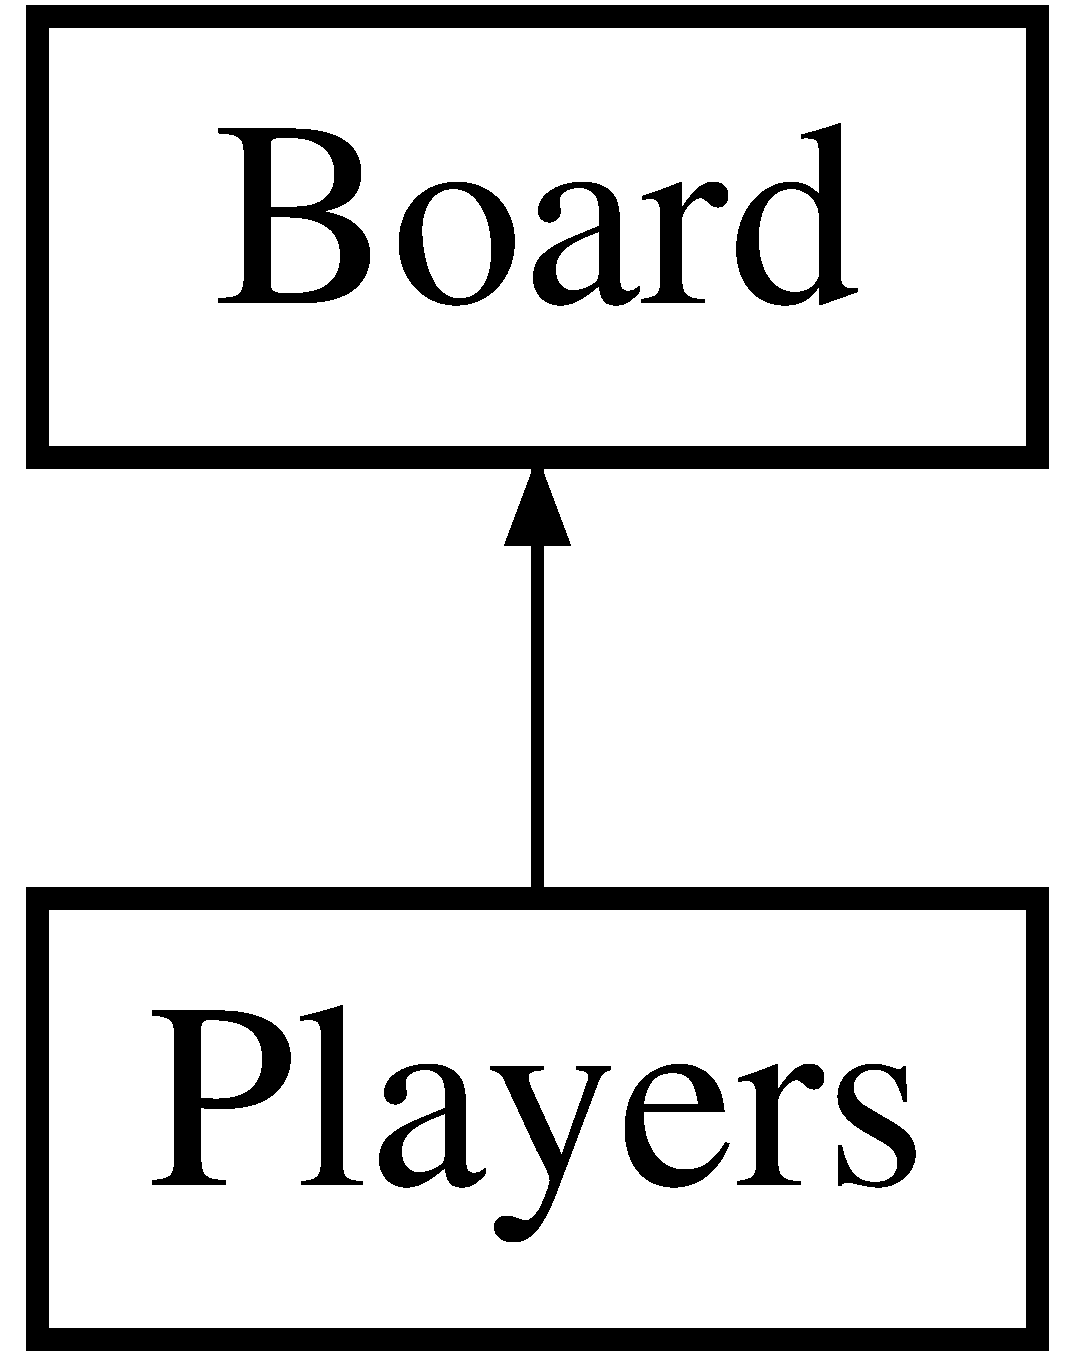
\includegraphics[height=2.000000cm]{class_players}
\end{center}
\end{figure}
\subsection*{Public Member Functions}
\begin{DoxyCompactItemize}
\item 
\hyperlink{class_players_a3ff1a0488140a54cc4e355716b9bef9d}{Players} ()
\item 
\hyperlink{class_players_a06057f5cdbb8c8837592d4c2c4489bb2}{Players} (int r, int c, int s)
\item 
\hyperlink{class_players_a550b03902064fa337ccf9f9f67b01d88}{$\sim$\+Players} ()
\item 
char $\ast$$\ast$ \hyperlink{class_players_a183f92c48a1bd651049188b8ab21f258}{get\+Player} ()
\item 
char $\ast$$\ast$ \hyperlink{class_players_ac93f72a2b68c2aa9175ee5134526b5e8}{get\+Enemy} ()
\end{DoxyCompactItemize}


\subsection{Detailed Description}


Definition at line 13 of file Players.\+h.



\subsection{Constructor \& Destructor Documentation}
\hypertarget{class_players_a3ff1a0488140a54cc4e355716b9bef9d}{\index{Players@{Players}!Players@{Players}}
\index{Players@{Players}!Players@{Players}}
\subsubsection[{Players}]{\setlength{\rightskip}{0pt plus 5cm}Players\+::\+Players (
\begin{DoxyParamCaption}
{}
\end{DoxyParamCaption}
)\hspace{0.3cm}{\ttfamily [inline]}}}\label{class_players_a3ff1a0488140a54cc4e355716b9bef9d}


Definition at line 19 of file Players.\+h.

\hypertarget{class_players_a06057f5cdbb8c8837592d4c2c4489bb2}{\index{Players@{Players}!Players@{Players}}
\index{Players@{Players}!Players@{Players}}
\subsubsection[{Players}]{\setlength{\rightskip}{0pt plus 5cm}Players\+::\+Players (
\begin{DoxyParamCaption}
\item[{int}]{r, }
\item[{int}]{c, }
\item[{int}]{s}
\end{DoxyParamCaption}
)\hspace{0.3cm}{\ttfamily [inline]}}}\label{class_players_a06057f5cdbb8c8837592d4c2c4489bb2}


Definition at line 20 of file Players.\+h.

\hypertarget{class_players_a550b03902064fa337ccf9f9f67b01d88}{\index{Players@{Players}!````~Players@{$\sim$\+Players}}
\index{````~Players@{$\sim$\+Players}!Players@{Players}}
\subsubsection[{$\sim$\+Players}]{\setlength{\rightskip}{0pt plus 5cm}Players\+::$\sim$\+Players (
\begin{DoxyParamCaption}
{}
\end{DoxyParamCaption}
)\hspace{0.3cm}{\ttfamily [inline]}}}\label{class_players_a550b03902064fa337ccf9f9f67b01d88}


Definition at line 22 of file Players.\+h.



\subsection{Member Function Documentation}
\hypertarget{class_players_ac93f72a2b68c2aa9175ee5134526b5e8}{\index{Players@{Players}!get\+Enemy@{get\+Enemy}}
\index{get\+Enemy@{get\+Enemy}!Players@{Players}}
\subsubsection[{get\+Enemy}]{\setlength{\rightskip}{0pt plus 5cm}char $\ast$$\ast$ Players\+::get\+Enemy (
\begin{DoxyParamCaption}
{}
\end{DoxyParamCaption}
)}}\label{class_players_ac93f72a2b68c2aa9175ee5134526b5e8}


Definition at line 86 of file Players.\+cpp.

\hypertarget{class_players_a183f92c48a1bd651049188b8ab21f258}{\index{Players@{Players}!get\+Player@{get\+Player}}
\index{get\+Player@{get\+Player}!Players@{Players}}
\subsubsection[{get\+Player}]{\setlength{\rightskip}{0pt plus 5cm}char $\ast$$\ast$ Players\+::get\+Player (
\begin{DoxyParamCaption}
{}
\end{DoxyParamCaption}
)}}\label{class_players_a183f92c48a1bd651049188b8ab21f258}


Definition at line 15 of file Players.\+cpp.



The documentation for this class was generated from the following files\+:\begin{DoxyCompactItemize}
\item 
\hyperlink{_players_8h}{Players.\+h}\item 
\hyperlink{_players_8cpp}{Players.\+cpp}\end{DoxyCompactItemize}

\chapter{File Documentation}
\hypertarget{_8dep_8inc}{\section{.dep.\+inc File Reference}
\label{_8dep_8inc}\index{.\+dep.\+inc@{.\+dep.\+inc}}
}

\hypertarget{_board_8cpp}{\section{Board.\+cpp File Reference}
\label{_board_8cpp}\index{Board.\+cpp@{Board.\+cpp}}
}
{\ttfamily \#include \char`\"{}Board.\+h\char`\"{}}\\*

\hypertarget{_board_8h}{\section{Board.\+h File Reference}
\label{_board_8h}\index{Board.\+h@{Board.\+h}}
}
\subsection*{Classes}
\begin{DoxyCompactItemize}
\item 
class \hyperlink{class_board}{Board}
\item 
class \hyperlink{class_board_1_1_invalid_input}{Board\+::\+Invalid\+Input}
\end{DoxyCompactItemize}

\hypertarget{_board_8o_8d}{\section{build/\+Debug/\+Cygwin\+\_\+4.x-\/\+Windows/\+Board.o.\+d File Reference}
\label{_board_8o_8d}\index{build/\+Debug/\+Cygwin\+\_\+4.\+x-\/\+Windows/\+Board.\+o.\+d@{build/\+Debug/\+Cygwin\+\_\+4.\+x-\/\+Windows/\+Board.\+o.\+d}}
}

\hypertarget{_check_winner_8o_8d}{\section{build/\+Debug/\+Cygwin\+\_\+4.x-\/\+Windows/\+Check\+Winner.o.\+d File Reference}
\label{_check_winner_8o_8d}\index{build/\+Debug/\+Cygwin\+\_\+4.\+x-\/\+Windows/\+Check\+Winner.\+o.\+d@{build/\+Debug/\+Cygwin\+\_\+4.\+x-\/\+Windows/\+Check\+Winner.\+o.\+d}}
}

\hypertarget{main_8o_8d}{\section{build/\+Debug/\+Cygwin\+\_\+4.x-\/\+Windows/main.o.\+d File Reference}
\label{main_8o_8d}\index{build/\+Debug/\+Cygwin\+\_\+4.\+x-\/\+Windows/main.\+o.\+d@{build/\+Debug/\+Cygwin\+\_\+4.\+x-\/\+Windows/main.\+o.\+d}}
}

\hypertarget{_players_8o_8d}{\section{build/\+Debug/\+Cygwin\+\_\+4.x-\/\+Windows/\+Players.o.\+d File Reference}
\label{_players_8o_8d}\index{build/\+Debug/\+Cygwin\+\_\+4.\+x-\/\+Windows/\+Players.\+o.\+d@{build/\+Debug/\+Cygwin\+\_\+4.\+x-\/\+Windows/\+Players.\+o.\+d}}
}

\hypertarget{_check_winner_8cpp}{\section{Check\+Winner.\+cpp File Reference}
\label{_check_winner_8cpp}\index{Check\+Winner.\+cpp@{Check\+Winner.\+cpp}}
}
{\ttfamily \#include $<$iostream$>$}\\*
{\ttfamily \#include \char`\"{}Check\+Winner.\+h\char`\"{}}\\*

\hypertarget{_check_winner_8h}{\section{Check\+Winner.\+h File Reference}
\label{_check_winner_8h}\index{Check\+Winner.\+h@{Check\+Winner.\+h}}
}
\subsection*{Classes}
\begin{DoxyCompactItemize}
\item 
class \hyperlink{class_check_winner}{Check\+Winner}
\end{DoxyCompactItemize}

\hypertarget{main_8cpp}{\section{main.\+cpp File Reference}
\label{main_8cpp}\index{main.\+cpp@{main.\+cpp}}
}
{\ttfamily \#include $<$cstdlib$>$}\\*
{\ttfamily \#include $<$iostream$>$}\\*
{\ttfamily \#include $<$iomanip$>$}\\*
{\ttfamily \#include $<$time.\+h$>$}\\*
{\ttfamily \#include $<$stdlib.\+h$>$}\\*
{\ttfamily \#include $<$fstream$>$}\\*
{\ttfamily \#include \char`\"{}Players.\+h\char`\"{}}\\*
{\ttfamily \#include \char`\"{}Check\+Winner.\+h\char`\"{}}\\*
\subsection*{Functions}
\begin{DoxyCompactItemize}
\item 
void \hyperlink{main_8cpp_a36ad170338d7feb540a9ce2f1f8bb1b0}{intro} ()
\item 
void \hyperlink{main_8cpp_a0f39d2caf1a4050f131b99f4e6aa3366}{print\+Board} (\hyperlink{class_players}{Players})
\item 
void \hyperlink{main_8cpp_ac4d66095eb7b3d2ee507bc7e2fc02236}{player\+Board} (int, int, char $\ast$$\ast$)
\item 
void \hyperlink{main_8cpp_a32a8ee32882627bc93ad1ef9a396aca2}{enemy\+Board} (int, int, char $\ast$$\ast$)
\item 
bool \hyperlink{main_8cpp_a105dccc974449c22a902770b3a211f10}{check\+Win} (int, int, int)
\item 
int \hyperlink{main_8cpp_a3c04138a5bfe5d72780bb7e82a18e627}{main} (int argc, char $\ast$$\ast$argv)
\end{DoxyCompactItemize}


\subsection{Function Documentation}
\hypertarget{main_8cpp_a105dccc974449c22a902770b3a211f10}{\index{main.\+cpp@{main.\+cpp}!check\+Win@{check\+Win}}
\index{check\+Win@{check\+Win}!main.\+cpp@{main.\+cpp}}
\subsubsection[{check\+Win}]{\setlength{\rightskip}{0pt plus 5cm}bool check\+Win (
\begin{DoxyParamCaption}
\item[{int}]{player, }
\item[{int}]{enemy, }
\item[{int}]{ships}
\end{DoxyParamCaption}
)}}\label{main_8cpp_a105dccc974449c22a902770b3a211f10}


Definition at line 319 of file main.\+cpp.

\hypertarget{main_8cpp_a32a8ee32882627bc93ad1ef9a396aca2}{\index{main.\+cpp@{main.\+cpp}!enemy\+Board@{enemy\+Board}}
\index{enemy\+Board@{enemy\+Board}!main.\+cpp@{main.\+cpp}}
\subsubsection[{enemy\+Board}]{\setlength{\rightskip}{0pt plus 5cm}void enemy\+Board (
\begin{DoxyParamCaption}
\item[{int}]{, }
\item[{int}]{, }
\item[{char $\ast$$\ast$}]{}
\end{DoxyParamCaption}
)}}\label{main_8cpp_a32a8ee32882627bc93ad1ef9a396aca2}
\hypertarget{main_8cpp_a36ad170338d7feb540a9ce2f1f8bb1b0}{\index{main.\+cpp@{main.\+cpp}!intro@{intro}}
\index{intro@{intro}!main.\+cpp@{main.\+cpp}}
\subsubsection[{intro}]{\setlength{\rightskip}{0pt plus 5cm}void intro (
\begin{DoxyParamCaption}
{}
\end{DoxyParamCaption}
)}}\label{main_8cpp_a36ad170338d7feb540a9ce2f1f8bb1b0}


Definition at line 267 of file main.\+cpp.

\hypertarget{main_8cpp_a3c04138a5bfe5d72780bb7e82a18e627}{\index{main.\+cpp@{main.\+cpp}!main@{main}}
\index{main@{main}!main.\+cpp@{main.\+cpp}}
\subsubsection[{main}]{\setlength{\rightskip}{0pt plus 5cm}int main (
\begin{DoxyParamCaption}
\item[{int}]{argc, }
\item[{char $\ast$$\ast$}]{argv}
\end{DoxyParamCaption}
)}}\label{main_8cpp_a3c04138a5bfe5d72780bb7e82a18e627}


Definition at line 32 of file main.\+cpp.

\hypertarget{main_8cpp_ac4d66095eb7b3d2ee507bc7e2fc02236}{\index{main.\+cpp@{main.\+cpp}!player\+Board@{player\+Board}}
\index{player\+Board@{player\+Board}!main.\+cpp@{main.\+cpp}}
\subsubsection[{player\+Board}]{\setlength{\rightskip}{0pt plus 5cm}void player\+Board (
\begin{DoxyParamCaption}
\item[{int}]{, }
\item[{int}]{, }
\item[{char $\ast$$\ast$}]{}
\end{DoxyParamCaption}
)}}\label{main_8cpp_ac4d66095eb7b3d2ee507bc7e2fc02236}
\hypertarget{main_8cpp_a0f39d2caf1a4050f131b99f4e6aa3366}{\index{main.\+cpp@{main.\+cpp}!print\+Board@{print\+Board}}
\index{print\+Board@{print\+Board}!main.\+cpp@{main.\+cpp}}
\subsubsection[{print\+Board}]{\setlength{\rightskip}{0pt plus 5cm}void print\+Board (
\begin{DoxyParamCaption}
\item[{{\bf Players}}]{a}
\end{DoxyParamCaption}
)}}\label{main_8cpp_a0f39d2caf1a4050f131b99f4e6aa3366}


Definition at line 284 of file main.\+cpp.


\hypertarget{_players_8cpp}{\section{Players.\+cpp File Reference}
\label{_players_8cpp}\index{Players.\+cpp@{Players.\+cpp}}
}
{\ttfamily \#include $<$iostream$>$}\\*
{\ttfamily \#include $<$stdlib.\+h$>$}\\*
{\ttfamily \#include \char`\"{}Players.\+h\char`\"{}}\\*

\hypertarget{_players_8h}{\section{Players.\+h File Reference}
\label{_players_8h}\index{Players.\+h@{Players.\+h}}
}
{\ttfamily \#include \char`\"{}Board.\+h\char`\"{}}\\*
\subsection*{Classes}
\begin{DoxyCompactItemize}
\item 
class \hyperlink{class_players}{Players}
\end{DoxyCompactItemize}

%--- End generated contents ---

% Index
\newpage
\phantomsection
\addcontentsline{toc}{chapter}{Index}
\printindex

\end{document}
